\begin{figure}[htbp]
\centering
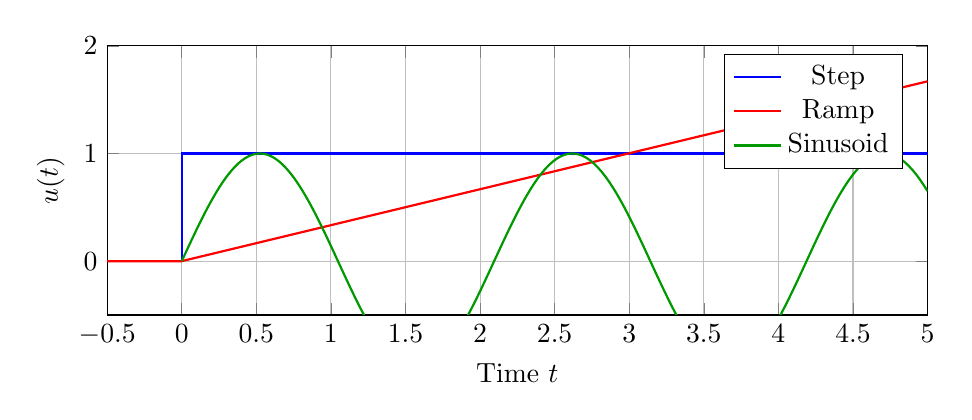
\begin{tikzpicture}
\begin{axis}[
    width=12cm, height=5cm,
    xlabel={Time $t$},
    ylabel={$u(t)$},
    xmin=-0.5, xmax=5,
    ymin=-0.5, ymax=2,
    legend pos=north east,
    grid=major,
    domain=0:5,
    samples=200
]
\addplot[blue, thick] coordinates {(-0.5,0) (0,0) (0,1) (5,1)};
\addlegendentry{Step}

\addplot[red, thick] coordinates {(-0.5,0) (0,0) (5,1.67)};
\addlegendentry{Ramp}

\addplot[green!60!black, thick] {sin(deg(3*x))};
\addlegendentry{Sinusoid}
\end{axis}
\end{tikzpicture}
\caption{Standard test inputs for system characterization.}
\label{fig:test_inputs}
\end{figure}
